\documentclass[a4paper]{article}

\usepackage{tikz}
\usetikzlibrary{bayesnet}

% name, --, caption, pos
\newcommand{\nofactor}[4]{
\node (#1) [factor, #2]  {};
\node (capt#1) [#4 of #1]{\footnotesize{#3}};
}

%shapename,  fitlist, caption
\newcommand{\namedgate}[3]{
\node (invisgate#1) [rectangle, draw, transparent,  fit=#2] {};
\node (gatecapt#1) [ above right=0 pt of invisgate#1.north west, xshift=-1pt ] {\footnotesize{#3}};
\node (#1) [rectangle,draw,dashed, inner sep=2pt, fit=(invisgate#1)(gatecapt#1)]{};

}

\begin{document}

\section{Latent dirichlet allocation}
\input{model_lda}

\section{Shared taste model}
\input{model_st}

\section{Citation influence model}
% model_citation_influence.tex
%
% Copyright (C) 2010,2011 Laura Dietz
% Copyright (C) 2012 Jaakko Luttinen
%
% This file may be distributed and/or modified
%
% 1. under the LaTeX Project Public License and/or
% 2. under the GNU General Public License.
%
% See the files LICENSE_LPPL and LICENSE_GPL for more details.

% Citation influence model
% Cite this model as 
% Laura Dietz, Steffen Bickel, Tobias Scheffer. 
% Unsupervised Prediction of Citation Influences. 
% In: Proceedings of International Conference on Machine Learning. 2007

%\beginpgfgraphicnamed{model-citation-influence}
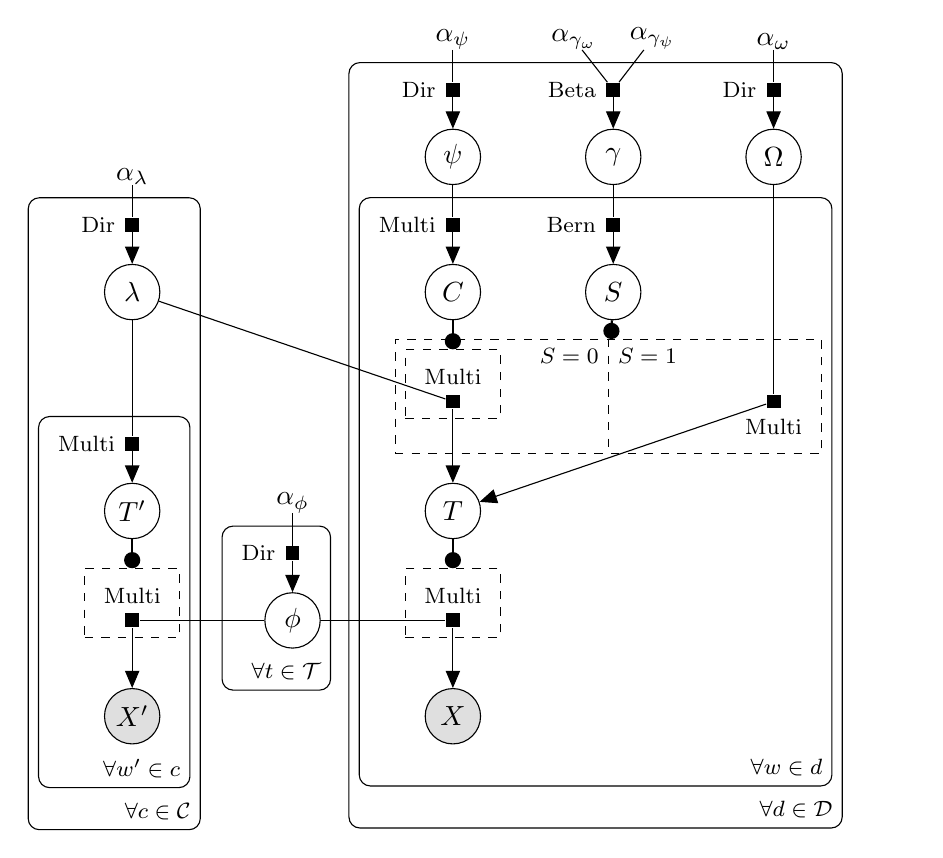
\begin{tikzpicture}

  % Layout the variables
  \matrix[row sep=0.5cm, column sep=1.2cm] (LDA)
  { %
    & %
    & %
    \node[latent] (psi)    {$\psi$} ; & %
    \node[latent] (gamma)  {$\gamma$} ; & %
    \node[latent] (omega)  {$\Omega$} ; & %
    \\
    \\
    \node[latent] (lambda) {$\lambda$} ; & %
    & %
    \node[latent] (C)      {$C$} ; & %
    \node[latent] (S)      {$S$} ; & %
    \\
    & %
    & %
    \factor       {T-f1}   {Multi} {} {}; & %
    & %
    \factor       {T-f2}   {below:Multi} {} {}; & %
    \\
    \node[latent] (T')     {$T'$} ; & %
    & %
    \node[latent] (T)      {$T$} ; & %
    \\
    \factor       {X'-f}   {Multi} {} {}; & %
    \node[latent] (phi)    {$\phi$} ; & %
    \factor       {X-f}    {Multi} {} {}; %
    \\
    \node[obs] (X')        {$X'$} ; & %
    & %
    \node[obs] (X)         {$X$} ;
    \\
  };

  % Remaining factors
  \factor[above=of T']     {T'-f}     {left:Multi} {} {}; %
  \factor[above=of lambda] {lambda-f} {left:Dir} {} {}; %
  \factor[above=of C]      {C-f}      {left:Multi} {} {}; %
  \factor[above=of S]      {S-f}      {left:Bern} {} {}; %
  \factor[above=of psi]    {psi-f}    {left:Dir} {} {}; %
  \factor[above=of gamma]  {gamma-f}  {left:Beta} {} {}; %
  \factor[above=of omega]  {omega-f}  {left:Dir} {} {}; %
  \factor[above=of phi]    {phi-f}    {left:Dir} {} {}; %

  % Hyperparameters
  \node[const, above=of lambda] (alambda) {$\alpha_\lambda$}; %
  \node[const, above=of phi]    (aphi)    {$\alpha_\phi$}; %
  \node[const, above=of psi]    (apsi)    {$\alpha_\psi$}; %
  \node[const, above=of gamma, xshift=-0.5cm] (agamma1)
  {$\alpha_{\gamma_\omega}$}; %
  \node[const, above=of gamma, xshift=0.5cm] (agamma2)
  {$\alpha_{\gamma_\psi}$}; %
  \node[const, above=of omega]  (aomega)    {$\alpha_\omega$}; %

  % Factor connections
  \factoredge {phi}               {X'-f}     {X'} ; %
  \factoredge {phi}               {X-f}      {X} ; %
  \factoredge {lambda}            {T'-f}     {T'} ; %
  \factoredge {lambda}            {T-f1}     {T} ; %
  \factoredge {omega}             {T-f2}     {T} ; %
  \factoredge {alambda}           {lambda-f} {lambda} ; %
  \factoredge {psi}               {C-f}      {C} ; %
  \factoredge {gamma}             {S-f}      {S} ; %
  \factoredge {apsi}              {psi-f}    {psi} ; %
  \factoredge {agamma1,agamma2}   {gamma-f}  {gamma} ; %
  \factoredge {aomega}            {omega-f}  {omega} ; %
  \factoredge {aphi}              {phi-f}    {phi} ; %

  % Gates
  \gate {X'-gate} {(X'-f)(X'-f-caption)} {T'} ; %
  \gate {X-gate}  {(X-f)(X-f-caption)}   {T} ; %
  \gate {T-gate}  {(T-f1)(T-f1-caption)} {C} ;
  \vgate {T-vgate} %
  {(T-gate)} {$S=0$} %
  {(T-f2)(T-f2-caption)} {$S=1$} %
  {S} ; %

  % Plates
  \plate {LDA1} { %
    (T')(T'-f)(T'-f-caption) %
    (X')(X'-gate) %
  } {$\forall w' \in c$} ; %

  \plate {LDA2} { %
    (LDA1) %
    (lambda)(lambda-f)(lambda-f-caption) %
  } {$\forall c \in \mathcal{C}$} ; %

  \plate {} { %
    (phi)(phi-f)(phi-f-caption) %
  } {$\forall t \in \mathcal{T}$} ; %

  \plate {P1} { %
    (X)(X-gate) %
    (T)(T-vgate) %
    (C)(C-f)(C-f-caption) %
    (S)(S-f)(S-f-caption) %
  } {$\forall w \in d$} ;

  \plate {} { %
    (P1) %
    (psi)(psi-f)(psi-f-caption) %
    (gamma)(gamma-f)(gamma-f-caption) %
    (omega)(omega-f)(omega-f-caption) %
  } {$\forall d \in \mathcal{D}$} ; %

\end{tikzpicture}
%\endpgfgraphicnamed

%%% Local Variables: 
%%% mode: tex-pdf
%%% TeX-master: "example"
%%% End: 


\section{Citation influence model with no topics}
% model_citation_influence.tex
%
% Copyright (C) 2010,2011 Laura Dietz
% Copyright (C) 2012 Jaakko Luttinen
%
% This file may be distributed and/or modified
%
% 1. under the LaTeX Project Public License and/or
% 2. under the GNU General Public License.
%
% See the files LICENSE_LPPL and LICENSE_GPL for more details.

% Citation influence model
% Cite this model as 
% Laura Dietz, Steffen Bickel, Tobias Scheffer. 
% Unsupervised Prediction of Citation Influences. 
% In: Proceedings of International Conference on Machine Learning. 2007

%\beginpgfgraphicnamed{model-citation-influence}
\begin{tikzpicture}

  % Layout the variables
  \matrix[row sep=0.5cm, column sep=1.2cm] (LDA)
  { %
    & %
    & %
    \node[latent] (psi)    {$\psi$} ; & %
    \node[latent] (gamma)  {$\gamma$} ; & %
    \node[latent] (omega)  {$\Omega$} ; & %
    \\
    \\
    \node[latent] (lambda) {$\lambda$} ; & %
    & %
    \node[latent] (C)      {$C$} ; & %
    \node[latent] (S)      {$S$} ; & %
    \\
    \factor       {X'-f}   {left:Multi} {} {}; & %
    & %
    \factor       {X-f1}   {Multi} {} {}; & %
    & %
    \factor       {X-f2}   {below:Multi} {} {}; & %
    \\
    \node[obs] (X')        {$X'$} ; & %
    & %
    \node[obs] (X)         {$X$} ;
    \\
  };

  % Remaining factors
  \factor[above=of lambda] {lambda-f} {left:Dir} {} {}; %
  \factor[above=of C]      {C-f}      {left:Multi} {} {}; %
  \factor[above=of S]      {S-f}      {left:Bern} {} {}; %
  \factor[above=of psi]    {psi-f}    {left:Dir} {} {}; %
  \factor[above=of gamma]  {gamma-f}  {left:Beta} {} {}; %
  \factor[above=of omega]  {omega-f}  {left:Dir} {} {}; %

  % Hyperparameters
  \node[const, above=of lambda] (alambda) {$\alpha_\lambda$}; %
  \node[const, above=of psi]    (apsi)    {$\alpha_\psi$}; %
  \node[const, above=of gamma, xshift=-0.5cm] (agamma1)
  {$\alpha_{\gamma_\omega}$}; %
  \node[const, above=of gamma, xshift=0.5cm] (agamma2)
  {$\alpha_{\gamma_\psi}$}; %
  \node[const, above=of omega]  (aomega)    {$\alpha_\omega$}; %

  % Factor connections
  \factoredge {lambda}            {X'-f}     {X'} ; %
  \factoredge {lambda}            {X-f1}     {X} ; %
  \factoredge {omega}             {X-f2}     {X} ; %
  \factoredge {alambda}           {lambda-f} {lambda} ; %
  \factoredge {psi}               {C-f}      {C} ; %
  \factoredge {gamma}             {S-f}      {S} ; %
  \factoredge {apsi}              {psi-f}    {psi} ; %
  \factoredge {agamma1,agamma2}   {gamma-f}  {gamma} ; %
  \factoredge {aomega}            {omega-f}  {omega} ; %

  % Gates
  \gate {X-gate}  {(X-f1)(X-f1-caption)} {C} ;
  \vgate {X-vgate} %
  {(X-gate)} {$S=0$} %
  {(X-f2)(X-f2-caption)} {$S=1$} %
  {S} ; %

  % Plates
  \plate {LDA1} { %
    (X'-f)(X'-f-caption) %
    (X')(X'-gate) %
  } {$\forall w' \in c$} ; %

  \plate {LDA2} { %
    (LDA1) %
    (lambda)(lambda-f)(lambda-f-caption) %
  } {$\forall c \in \mathcal{C}$} ; %

  \plate {P1} { %
    (X)(X-gate) %
    (T)(T-vgate) %
    (C)(C-f)(C-f-caption) %
    (S)(S-f)(S-f-caption) %
  } {$\forall w \in d$} ;

  \plate {} { %
    (P1) %
    (psi)(psi-f)(psi-f-caption) %
    (gamma)(gamma-f)(gamma-f-caption) %
    (omega)(omega-f)(omega-f-caption) %
  } {$\forall d \in \mathcal{D}$} ; %

\end{tikzpicture}
%\endpgfgraphicnamed

%%% Local Variables: 
%%% mode: tex-pdf
%%% TeX-master: "example"
%%% End: 


\end{document}
